% To add an image or include a .tex file you need to add
% \CWD
% to the relative (to the main document) path.
%
% Example:
% \begin{figure}
%   \centering
%   \includegraphics{\CWD/images/example.pdf}
% \end{figure}

Um sapo está no pântano, na frente de um rio. No rio há $N$ vitórias-régias, organizadas em uma sequência, da esquerda para a direita. O sapo sabe que, ao pular da vitória-régia $A$ para a vitória-régia $B$, a $A$ afunda para sempre no rio. Além disso, da $i$-ésima vitória-régia o sapo gasta $x_i$ de energia para pular para a esquerda (\textbf{independente do tamanho do pulo}), ou $y_i$ para a direita.

O sapo, então, por diversão, irá escolher uma das vitórias-régias, pular nela, e depois pular para \textbf{todas as outras antes de sair do rio}, decidindo em cada momento pular para a esquerda ou direita. Como ele tem medo de cair no rio, em cada pulo, ele \textbf{sempre pula para a vitória-régia mais próxima na direção escolhida que ainda não afundou}. O sapo quer afundar todas as vitórias-régia dessa maneira, e, depois, pular para fora do rio. Se o caminho do sapo termina na posição $i$, o custo de pular dessa última vitória-régia para fora do rio é o mínimo entre $x_i$ e $y_i$.

\begin{figure}[H]
  \centering
  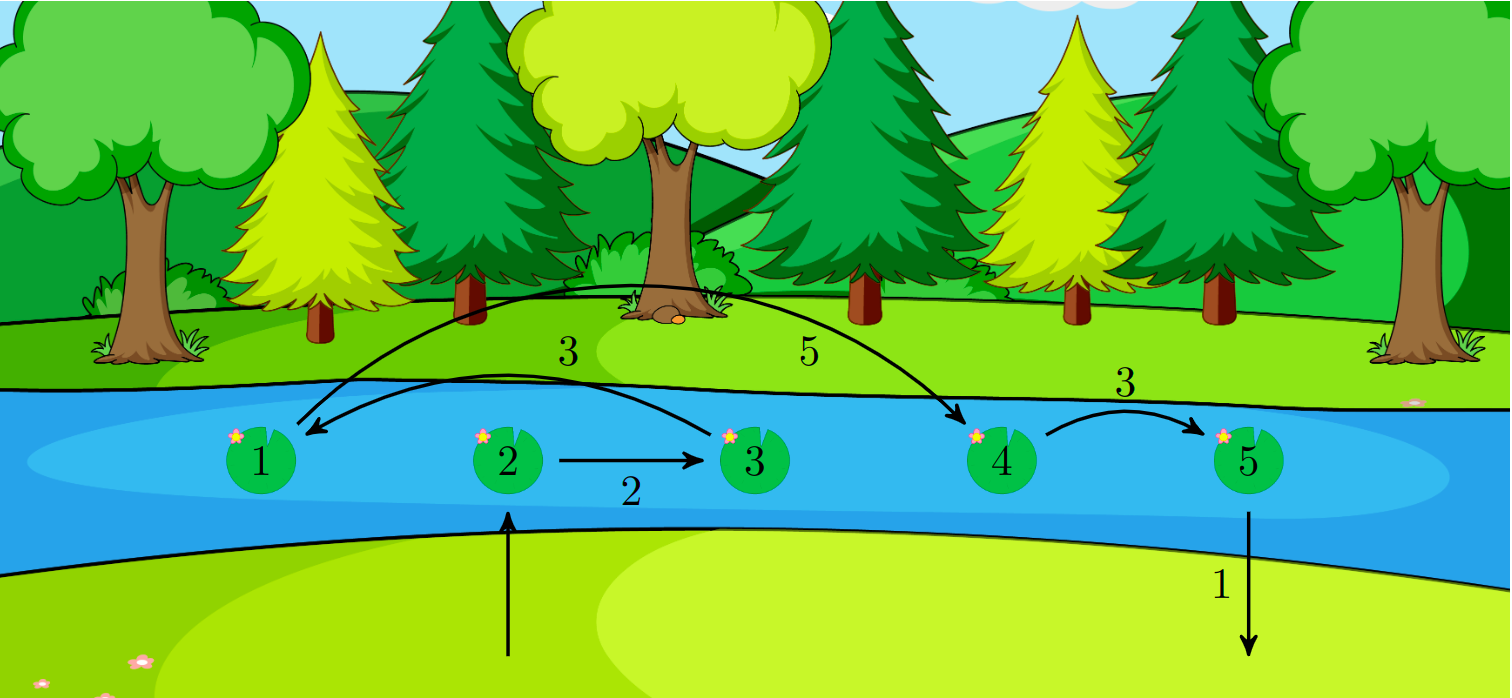
\includegraphics[scale=0.15]{\CWD/img/image.png}
  \caption{Representação do exemplo. A energia gasta é $2+3+5+3+1=14$.}
\end{figure}

Ajude o sapo a descobrir alguma sequência de vitórias-régia que minimiza a energia total gasta.

%
% For input, use one of the following
%

\section*{Entrada}

A primeira linha da entrada contém um inteiro $1 \leq N \leq 10^5$, a quantidade de vitórias-régia no lago. As próximas $N$ linhas possuem dois inteiros $1 \leq x_i, y_i \leq 10^9$, o quanto de energia que o sapo gasta para pular da $i$-ésima vitória-régia para a esquerda ou direita, respectivamente.

%
% For output, use one of the following
%

\section*{Saída}

Imprima uma sequência de índices que descreve uma sequência de pulos que minimiza a energia total gasta pelo sapo. Se houver várias soluções, imprima qualquer uma delas.

\section*{Restrições}

\begin{itemize}
\item $ 1 \leq N \leq 10^5$.
\item $1 \leq x_i, y_i \leq 10^9$.
\end{itemize}

%\sampleio will look for files named sample-n.in and sample-n.sol (where n is 1, 2, 3...)
%in the documents directory and include them as samples.

\exemplo
